\lab{Graphical User Interface}{GUI}
\label{lab:GUI}
\objective{Explain how to implement a GUI in python using PyQt.  Instruct how to create a basic GUI with standard features.}

\section*{Introduction}
\subsection*{Graphical User Interfaces and PyQt}
GUI stands for Graphical User Interface.  A GUI is an application that allows users to control a program through manipulation of graphical objects such as buttons, sliders, text boxes, and so forth.  In Python, we can use the PyQt toolkit to build GUIs.  From PyQt, we import the QtGui module which will allow us to implement the graphics as well as the interface itself. QtGui extends the module QtCore.  While most of what we do here only uses QtGui, occasionally QtCore will also be needed. 

To demonstrate the main ideas behind building a GUI, we will first create a simple program that displays inputted text. Then we will complete the MatrixCalculator GUI.  As you read, follow along by typing the code into a text editor and running it from your command line (use the command "python filename.py"). Hands-on experience is the best way for GUI concepts to solidify.

\subsection*{QMainWindow}
To become familiar with the basics behind GUIs, we will first build a very simple application.  Our Printer class will inherit from the QMainWindow class, which provides a main application window with support for useful things like a menu bar, toolbars, and animation.

\begin{lstlisting}
from PyQt4 import QtGui, QtCore

class Printer(QtGui.QMainWindow):
	# This class inherits from the QWidget class found in the QtGui module.
	def __init__(self):
		# Call the __init__ method from QMainWindow, the class Printer is sub-classed from (its "super" class).
		super(Printer, self).__init__()
		self._initUI()
	
	def _initUI(self):
		# Our constructor
		self.show()

\end{lstlisting}

\subsection*{Creating Instance of GUI}
To launch the GUI, we need a main function which will run when the program is executed.  In the main function, we create an instance of the GUI in the following manner.  Note we must import sys in order to do this.
\begin{lstlisting}
import sys

if __name__== "__main__":
    app = QtGui.QApplication(sys.argv)
    p = Printer()
    sys.exit(app.exec_())
\end{lstlisting}

If we were to run the program at this point (using "python filename.py" in the terminal), a completely blank GUI instance would be created.  Let us add widgets to our main window.

\section*{Widgets}
\emph{Widgets} are what make the magic happen in GUIs.
In Qt, widgets are objects that represent various elements of a GUI.
They keep track of drawing and refreshing the graphical display of the elements, abstracting the behavior of the elements, and defining ways to interact with other widgets.
When you push a button or enter text, widgets are what notice and respond accordingly.
In our \li{Printer} class, we will use \li{QTextEdit}, \li{QLabel}, and \li{QPushButton}.

\subsection*{Organization}
We can organize our widgets on the screen using layouts.  A QHBoxLayout, for instance, allows you to align widgets horizontally, while a QVBoxLayout stacks them vertically.  You can also arrange them into grids of arbitrary dimensions using QGridLayout.  QMainWindow has a solitary central widget.  We will put our widgets into one layout, set that layout on a generic QWidget, and then assign that widget to the central widget.  To create the layout and the central widget, we add the following to the constructor, above the call to \li{self.show}: 
\begin{lstlisting}
def _initUI(self):
	# Creates the layout of the GUI.
	layout = QtGui.QVBoxLayout()

	# Creates a QWidget that we will use as our central widget.
	window = QtGui.QWidget()
	window.setLayout(layout)
	self.setCentralWidget(window)
\end{lstlisting}

\subsection*{Text Box}
In order to receive user input, we need a text box.  We will use a QTextEdit widget.  The user's input will be displayed as a label.  Create a text box and a label and add them to the layout with the following code, sometime before setting the layout of \li{window}:
\begin{lstlisting}
def _initUI(self):
	# Creates the output textbox and adds it to the layout.
	self.userInput = QtGui.QTextEdit("Input here")
	self.output = QtGui.QLabel("Output here")
	layout.addWidget(self.userInput)
	layout.addWidget(self.output)
	
\end{lstlisting}


Note: Self is used to declare member variables.  You only need to declare an object with self if you intend to access that object from a member function of your class.  In this example, we do not declare the layouts with self because as soon as we assign the layout to the central widget we don't need to access them again.

\subsection*{Button}
Next we add a button to our GUI.  This will be done in the constructor, just as with the text box.
\begin{lstlisting}
# Creates a push button.
self.Button = QtGui.QPushButton("Enter")
layout.addWidget(self.Button)
\end{lstlisting}

At this point, the GUI has a text box, a label, and a button.  However, if the button is pressed, nothing happens.  We need to add functionality to our button and text box.

\subsection*{Add Functionality}
Now that we have our widgets, we need to tell them how to communicate.
Qt uses a system of \emph{signals} and \emph{slots}.
When a button is pushed or when text is entered, a widget throws a \emph{signal}.
We can specify which slot catches the signal.
In this case, the signal being thrown is the button being clicked. We want a function that catches the signal and updates the displayed text.  In order to add functionality to the button, add the following to the constructor:
\begin{lstlisting}
self.Button.clicked.connect(self.clickButton)
\end{lstlisting}
\li{clickButton} is a method that will be declared inside the \li{Printer} class.  Once the button is pressed, the method clickButton will be called.  This method will set the text of our QLabel to be whatever is currently in the text box.
\begin{lstlisting}
def clickButton(self):
	message = self.userInput.toPlainText()
	self.output.setText(message)
\end{lstlisting}
\begin{problem}
Create a GUI with a button, text box, and label that will display the contents of the text box in the label once the button is pressed.
\label{prob:basicGUI}
\end{problem}

\section*{Important Widgets}
In the MatrixCalculator, we become acquainted with several other widgets.

\subsection*{Menu Bar}
It is very common for GUIs to have a menu bar.  The QMainWindow class has a member function which generates one and puts it at the top of the window.  It will be empty to begin with.  We can add menu objects to it.  We can then add menus to the menus if we want, creating submenus to arbitrary levels.  At the bottom of the menu tree is an Action.  Action objects throw signals, and we connect the Actions to functions just like we did with the button.

In MatrixCalculator, we add Actions to import a matrix into the table.  The file spec.py describes the format for a matrix file.

\subsection*{Other Widgets}
QSpinBoxes allow users to enter in a number, either by typing it in, by clicking in the QSpinBox and then pressing the up and down arrow keys, or by clicking arrows on the side of the QSpinBox.  We use QSpinBoxes to define the dimensions of our matrix.

A QRadioButton is a circular button that is either off or on.  We use one of these to fill empty cells in our table with 0s.

A QComboBox widget is a drop down list of options.  In MatrixCalculator, we have a QComboBox which contains the different operations that the calculator will perform.

Refer to \ref{fig:widgets} to see what some of these widgets and others look like.  

\begin{figure}
\label{fig:widgets}
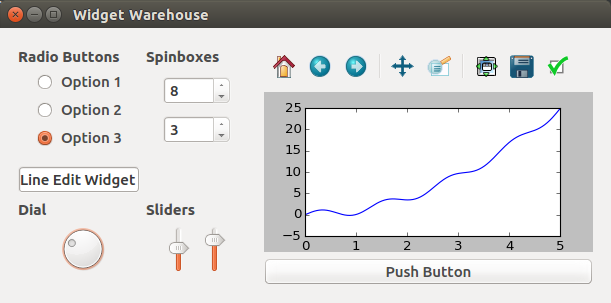
\includegraphics[width=\textwidth]{widgetwarehouse.png}
\caption{Several useful widgets.}
%TODOTo see an example using matplotlib in a GUI, refer to the file TODO

\end{figure}

\begin{problem}
Complete the MatrixCalculator class that is provided in spec.py by:
\begin{enumerate}
\item Adding a QComboBox to the GUI.  Call it matrixFunction, so as to match the rest of the provided code.
\item Add options to the QComboBox to calculate the determinant, inverse, and multiplication.  To be consistent with the rest of the class, call these "Determinant," "Inverse," and "Multiplication."
\item Implement the determinant and inverse function in \li{clickCalculate}.  Multiplication is already implemented.  Hint: Use the standard NumPy commands.
\item Display the proper output in the textbox.
\end{enumerate}
\end{problem}

\subsection*{Visibility}
Sometimes we want a widget to be invisible depending on certain conditions within the application.  In MatrixCalculator, there is a table for a second matrix, but we only want this to be visible when the Multiplication option is selected in the QComboBox.  You can call \li{setVisible} on any widget.  This function takes a boolean.  We include a method to update the display whenever the QComboBox matrixFunction is activated.

\section*{Documentation}
There are many different widgets that can be used in a variety of settings.  For a list of useful widgets see \href{http://doc.qt.io/qt-4.8/widgets-and-layouts.html}{link}.
Note: PyQt is the Python binding of the cross-platform toolkit Qt, which is written in C++.  Thus the official documentation is also in C++.  

For a really comprehensive list of widgets see \href{http://pyqt.sourceforge.net/Docs/PyQt4/qtgui.html}{link}.


\begin{problem}
Create your own GUI.  You may make the GUI to display an old lab in an interesting way.  Some suggestions are Numerical Derivatives, Image Segmentation, SVD, or Convolution.  Or you may make your own GUI.  Include at least 5 widgets.
\end{problem}

\begin{comment}

\begin{lstlisting}
from PySide import QtGui, QtCore

class Printer(QtGui.QWidget):
	def __init__(self):
		super(Printer, self).__init__()
		# Call the _initUI function.
		self._initUI()
	
	def _initUI(self):
		'''Creates the widgets and tells them how to interact.'''
		
		# Create a class variable called textBar that is a QLineEdit widget.
		self.textBar = QtGui.QLineEdit()
		# Create a class variable called label that is a QLabel widget.
		self.label = QtGui.QLabel()

\end{lstlisting}



\begin{lstlisting}
from PySide import QtGui, QtCore

class Printer(QtGui.QWidget):
	def __init__(self):
		super(Printer, self).__init__()
		self._initUI()

	def _initUI(self):
		self.textBar = QtGui.QLineEdit()
		self.label = QtGui.QLabel()
		
		# When return is pressed in the textBar, it sends a signal and goes into the function updateText.
        # self.textBar accesses the textBar object.
        # returnPressed defines the inputted signal.
        # connect links the signal to the method later defined in this class: updateText.
		self.textBar.returnPressed.connect(self.updateText)
	
		
	def updateText(self):
	'''Updates what text is displayed and clears the textBar'''
		self.label.setText(self.textBar.displayText())
		self.textBar.clear()

\end{lstlisting}

Next, we need to set the layout and create a function that can be called from the command line.

\begin{lstlisting}
from PySide import QtGui, QtCore
import sys

class Printer(QtGui.QWidget):
	def __init__(self):
		super(Printer, self).__init__()
		self._initUI()

	def _initUI(self):
		self.textBar = QtGui.QLineEdit()
		self.label = QtGui.QLabel()
		
		self.textBar.returnPressed.connect(self.updateText)
	
		# Create a vertical box layout.
		# This will stack all widgets added to it vertically.
		vbox = QtGui.QVBoxLayout()
		# Add textBar as a widget and display it on the first row (0) in the first column (0).
        vbox.addWidget(self.textBar, 0, 0)
		vbox.addWidget(self.label, 1, 0)
		
		# Assemble the layout.
		self.setLayout(vbox)
		# Tell the dimensions of the vbox.
		# The first two numbers indicate placement on the screen while the second two represent the dimensions.
		self.setGeometry(50, 50, 200, 200)
		self.setWindowTitle("Simple Printer")
		self.show()
	
	def updateText(self):
		self.label.setText(self.textBar.displayText())
		self.textBar.clear()
		
def main():
	# Create a QApplication.
    # Note that if you are working in IPython Notebook, you need to restart your kernel before running the program, or a RuntimeError will occur.
	app = QtGui.QApplication(sys.argv)
	# Create a Printer object.
    # Since _initUI is called in the constructor, the GUI will appear and run.
	p = Printer()
	sys.exit(app.exec_())
if __name__ == "__main__":
	main()

\end{lstlisting}

\begin{problem}
Create a simple graphical user interface that will solve the quadratic formula given the necessary parameters.
Make the GUI look similar to the one below.
\begin{figure}[H]
\centering
\end{comment}
\begin{comment}
\begin{subfigure}[b]{.49\textwidth}
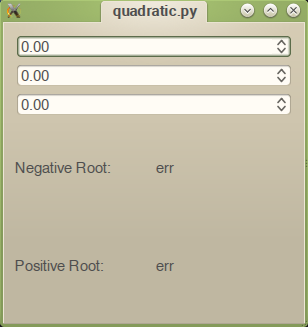
\includegraphics[width=\textwidth]{quadratic_view.png}
\end{subfigure}
\end{comment}
\begin{comment}
\begin{subfigure}[b]{.49\textwidth}
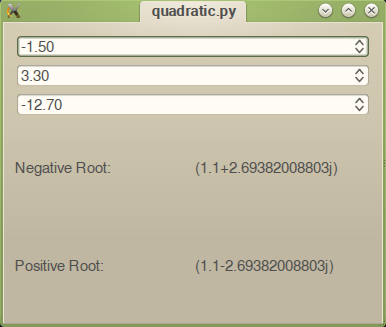
\includegraphics[width=\textwidth]{quadratic_view2.png}
\end{subfigure}
\end{figure}
The widgets that you will need are: \li{QDoubleSpinBox}, \li{QLabel}, \li{QGridLayout}, and \li{QVBoxLayout}. You may also want to import the cmath module in order to calculate complex solutions.
You can view the documentation for these classes, including all their methods and signals, at \url{http://qt-project.org/doc/qt-4.8/classes.html}
\label{prob:quadCalc}
\end{problem}


\section*{Specifications}

The following is a guideline for your solutions.

\begin{lstlisting}
import sys
from PySide import QtGui, QtCore

class People(object):
	pass
	
class ComplexNumber(object):
	pass
	
class QuadraticCalculator(QtGui.QWidget):
	pass
\end{lstlisting}
\end{comment}
